
\subsection{研究意义}
波动方程是二阶双曲型偏微分方程\cite{bedford1994},可用于描述地震波、水波、电磁波等自然界中的波动现象,广泛的应用于无损检测、地震预测、生物医学成像等各个工程领域。
发展波动方程的高精度分析方法将有助于提升如无损检测准确率、医学成像精度等。
由于实际工程问题中通常涉及复杂几何区域、材料非均质等一系列问题,采用理论分析手段研究波动问题难以获得解析解。于是,数值仿真分析成为了研究波动方程的重要工具。
在波动问题的主流数值分析方法中,时间域和空间域将独立离散为有限个分布节点用于近似位移变量,其中空间域通常采用基于变分原理的弱形式进行离散分析,如有限元法等。
在变分原理的帮助下,基于弱形式型的方法具有求解精度高、稳定性强的特点,适用于复杂空间几何构型。
而时间域则采用基于微分方程的强形式进行离散分析,如有限差分法等。
该类方法通常采用迭代形式进行程序实现,实现过程简单高效。
但基于强形式型的方法在计算精度和稳定性方面均低于基于弱形式型的方法,计算误差将随着迭代步的增加而累积增大。

波动方程数值分析方法构建的另一种思路是将时间域作为第四维空间,与时空间域进行混合离散,并采用基于哈密顿变分原理的弱形式进行求解。
该类方法将提升整体的求解精度,有利于时空区域自适应节点加密过程。
求解过程无需进行迭代,可采用整体并行计算求解提高效率。
然而自上世纪九十年代Hughes首次采用时空混合离散结合间断伽辽金法求解波动问题\cite{hughes1988}以来,该类方法发展缓慢。
\textbf{
主要的原因是该方法并不能适用于任意节点分布情况,导致其未能广泛应用于复杂的实际工程问题中,阻碍了时空混合离散伽辽金法的发展。
}
造成时空混合离散伽辽金法无法适用任意节点分布情况的原因主要有三点:

首先是\textbf{时域末端虚位移本质边界条件的施加问题}。
波动方程的时空混合离散伽辽金法通过哈密顿变分原理建立相对应的弱形式,
如图 \ref{fg:hamilton} 所示,哈密顿原理要求虚位移$\delta q$在初始时刻$t_0$和末端时刻$t_1$为零,即$\delta q(t_0)=\delta q(t_1)=0$,以等价于欧拉--拉格朗日方程\cite{arnold1978}。
在传统边值问题中,虚位移本质边界条件通常伴随着位移本质边界条件。
当采用伽辽金法进行求解时,即虚位移和位移采用相同的离散方式,位移及其虚位移涉及本质边界条件的自由度数量相同。
采用矩阵压缩技术直接施加本质边界条件时,可保持刚度矩阵为方阵且可逆。
然而,波动方程在时间维度上属于初值问题,即已知初始时刻位移和速度,$q(t_0)=q_0,\dot q(t_0) = \dot q_0$,时域末端边界条件未知。
如图 \ref{fg:direct} 所示,直接施加初始时刻位移边界条件将填补末端时刻虚位移为零造成刚度矩阵却是的部分。
而初始时刻虚位移不再要求为零,初始时刻速度边界条件可在此处作为自然边界条件施加。
但该方法可实施的前提是\textbf{涉及初始时刻和末端时刻的自由度数量需要保持一致,并不适用于任意节点分布情况。}
间断伽辽金法则是在弱形式中增加了哈密顿原理时域边界条件相关项,以规避虚位移本质边界条件的施加。
但是,该方法需要在时域上采用如图 \ref{fg:slab} 所示的分块离散以保证整体求解稳定性。
\textbf{时域分块网格不仅限制了节点布置,而且在时域块状边界处采用非连续的位移进行近似,增加位移自由度数量。}


\begin{figure}[!h]
    \centering 
    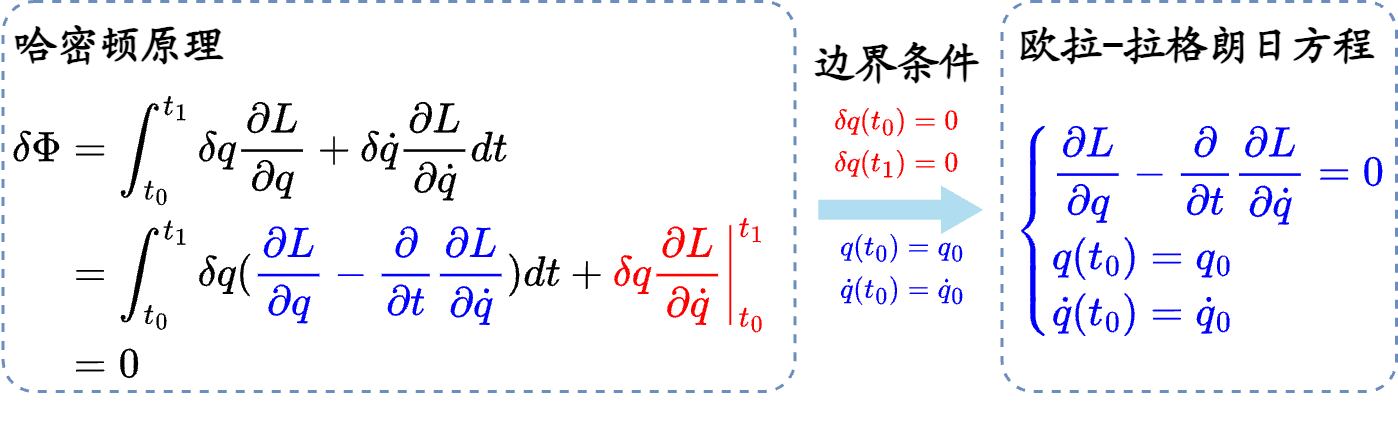
\includegraphics[width=\textwidth]{figures/Hamilton.png}
    \caption{哈密顿原理与欧拉--拉格朗日方程等价性}
    \label{fg:hamilton}
\end{figure}

\begin{figure}[!h]
    \centering 
    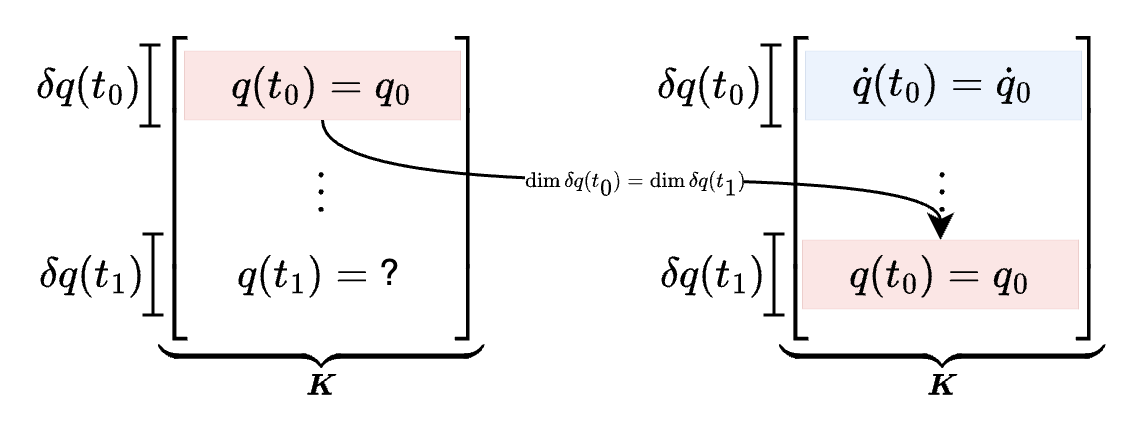
\includegraphics[width=0.8\textwidth]{figures/stiffness.png}
    \caption{直接施加时域末端虚位移本质边界条件}
    \label{fg:direct}
\end{figure}

\begin{figure}[!h]
    \centering 
    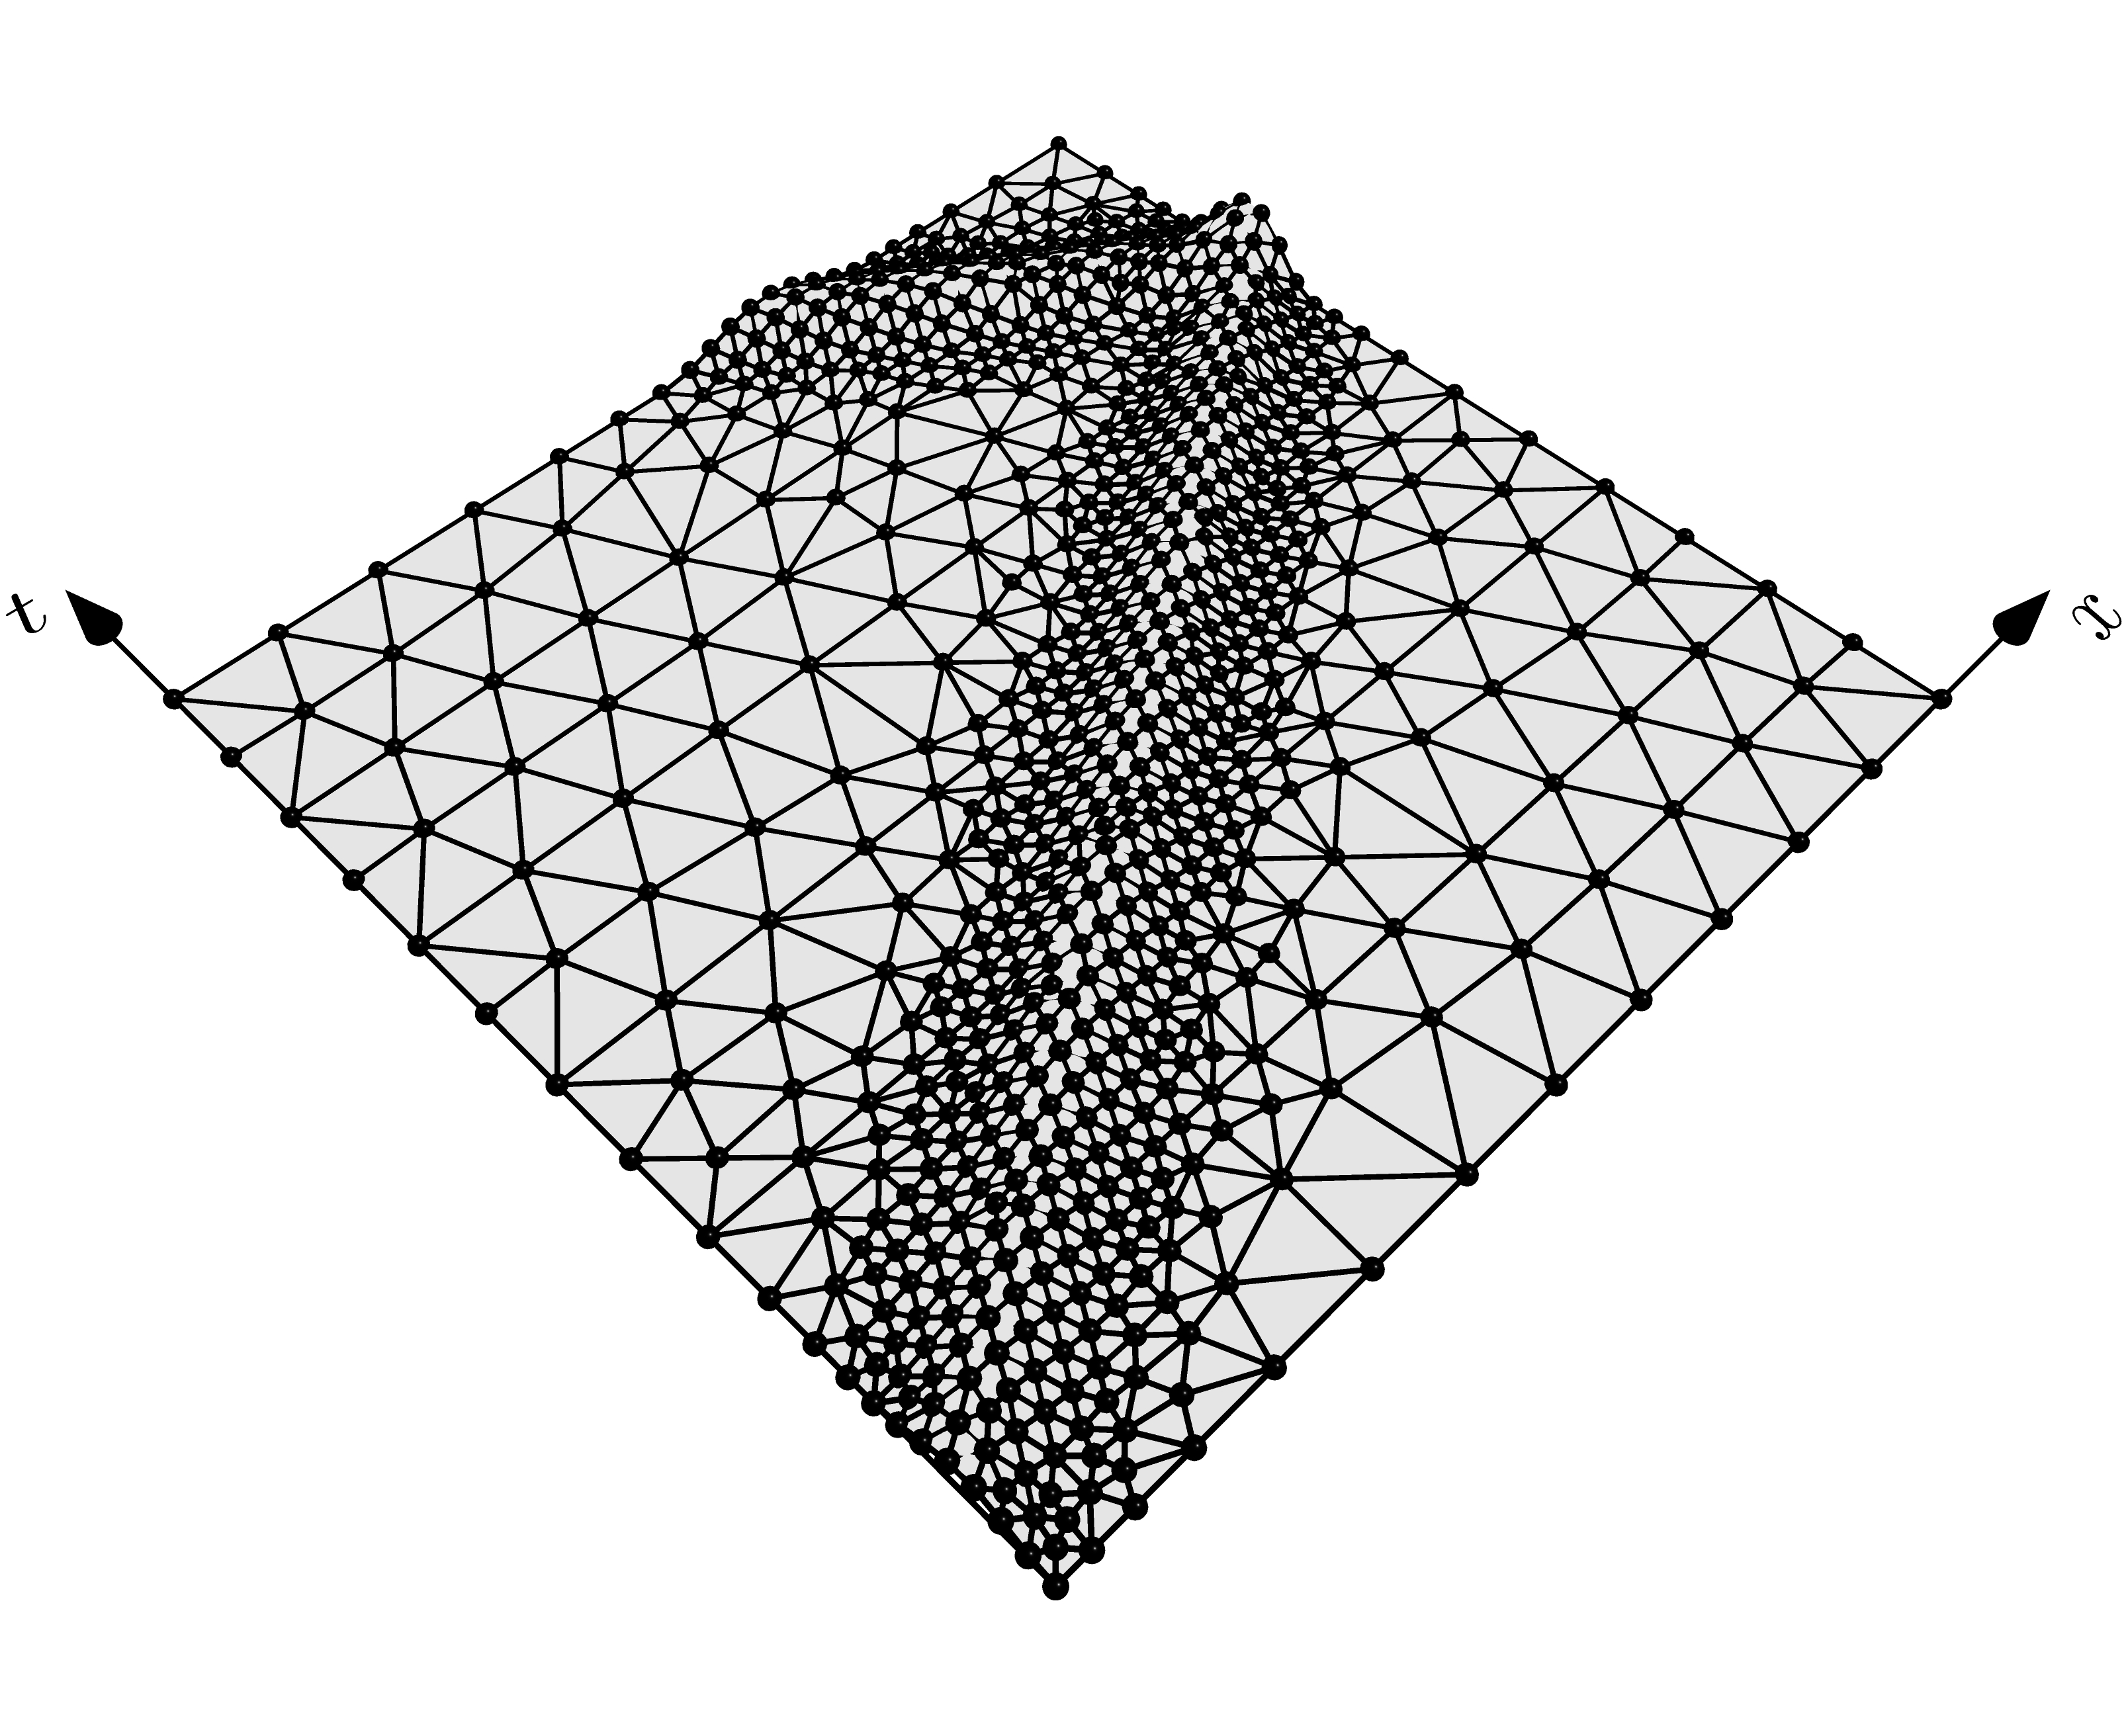
\includegraphics[width=0.8\textwidth]{figures/wave.png}
    \caption{时空混合离散间断伽辽金法}
    \label{fg:slab}
\end{figure}

% \begin{equation*}
% \begin{split}
% 	\delta \Phi&=\int_{t_0}^{t_1} \delta q \frac{\partial L}{\partial q} + \delta \dot q \frac{\partial L}{\partial \dot q} dt\\ &=\int_{t_0}^{t_1} \delta q({\color{blue}\frac{\partial L}{\partial q} - \frac{\partial}{\partial t}\frac{\partial L}{\partial \dot q}}) dt + {\color{red}\delta q \left . \frac{\partial L}{\partial \dot q}\right \vert_{t_0}^{t_1}}\\&= 0
% \end{split}
% \xrightarrow{{\color{red}\delta q(t_0)=\delta q(t_1)=0}}
% \color{blue}\left \{\begin{split}&\frac{\partial L}{\partial q} - \frac{\partial}{\partial t}\frac{\partial L}{\partial \dot q}=0\\& q(t_0) = q_0,\;\dot q(t_0) = \dot q_0\end{split}\right .
% \end{equation*}

其次是\textbf{空间域和时间域离散节点间距不匹配引起的数值色散问题}。

发展适用于任意节点分布的时空混合离散伽辽金法……

本项目

\subsection{国内外研究现状及发展动态}

\vspace{-5pt}

\begin{REF}
	\subsection*{参考文献}
	\vspace{-50pt}
	\bibliographystyle{gbt7714-2005-numerical}
	\bibliography{ref}%参考文献
\end{REF}

\newpage%自己判断是否需要
